
% To trzeba wypelnic swoimi danymi
\title{Distributed computing for fun and profit}

% autor(zy)
\author{Michał Zochniak}
\nrindeksu{221224}
% wstawienie zdjecia
\zdjecie{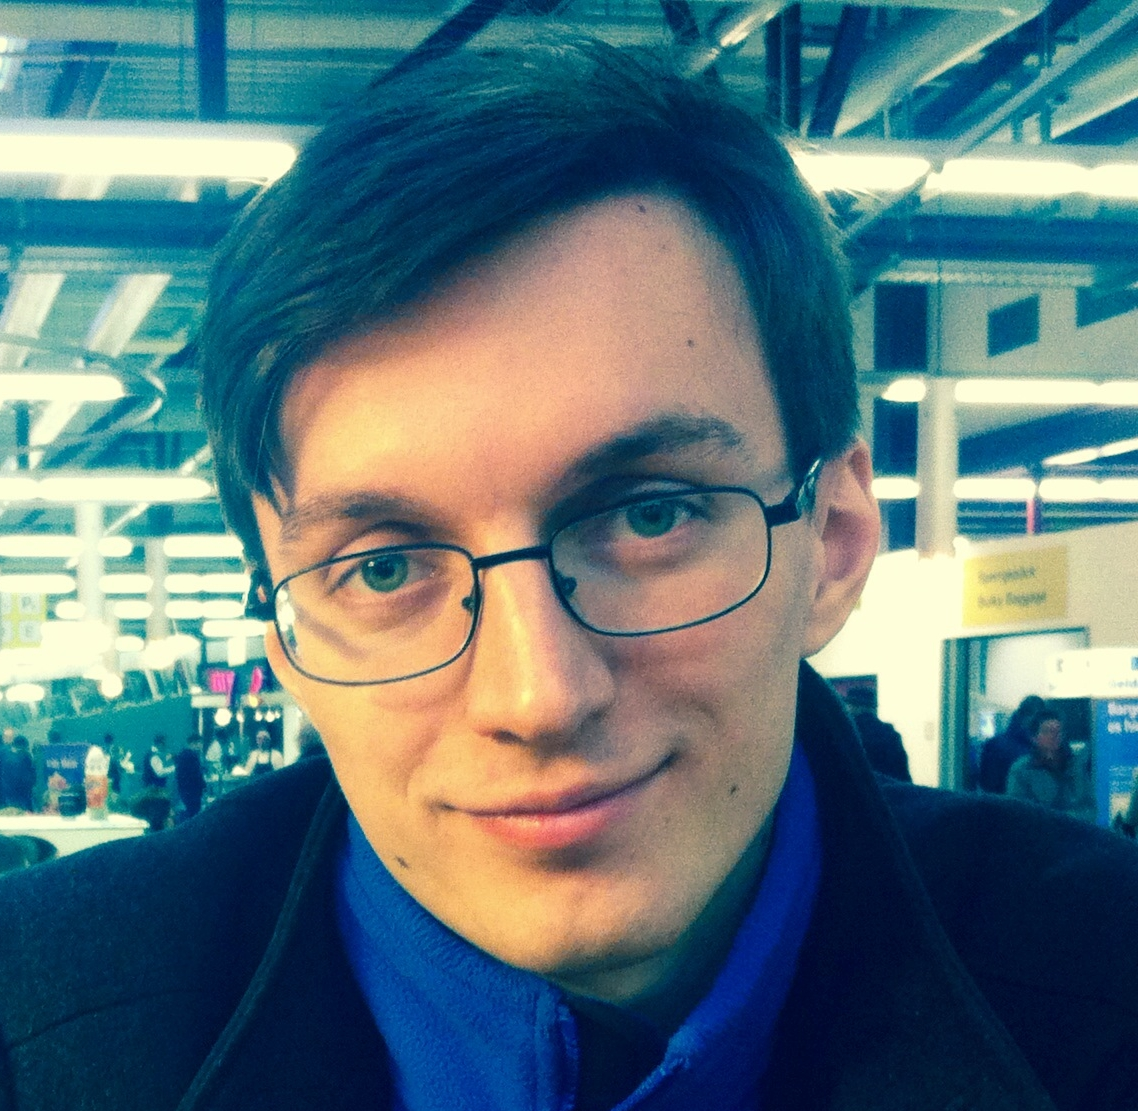
\includegraphics[width=4cm]{zdjecie.jpg}}

\opiekun{dr hab inż. Bartosz Sawicki}
% opcjonalnie: \konsultant{prof. Dzielny Konsultant}
\terminwykonania{10 czerwca 2014} % data złożenia - pokazana na stronie tytułowej
\datawydaniatematu{5 marca 2013}
\rokakademicki{2013/2014}

\streszczenie{
    Celem pracy dyplomowej było stworzenie systemu do przeprowadzania zdalnych testów użyteczności serwisów internetowych. Głównym założeniem systemu była możliwość uczestniczenia w testach użyteczności zdalnie (,,bez wychodzenia z domu'') oraz bez konieczności instalacji dodatkowego oprogramowania na komputerach testerów. Zaimplementowany w ramach pracy system pozwala na zdefiniowanie scenariuszy testowych oraz na przeprowadzenie testów użyteczności których wynikiem są raporty testowe.

    Raporty z przebiegu testu tworzone są przy użyciu serwera proxy który jest w stanie przechwytywać ruch między testerem a testowanym serwisem internetowym. Opracowana została metoda identyfikowania poszczególnych sesji testowych za pomocą ,,wstrzykiwania cookie'' przy rozpoczęciu sesji. Za pomocą proxy, strony HTML testowanego serwisu dekorowane są kodem JavaScript który przechwytuje zdarzenia takie jak kliknięcia myszą lub wypełnianie pól formularzy. Opracowane oraz opisane zostały trzy metody przechwytywania zdarzeń, jedna z nich została zaimplementowana w systemie.

    Praca zawiera specyfikację funkcjonalną oraz specyfikację niefunkcjonalną systemu. Specyfikacja funkcjonalna przedstawia główne założenia aplikacji, dodatkowo wzbogacona jest o makiety interfejsów użytkownika. Specyfikacja niefunkcjonalna opisuje sposób podziału systemu na moduły oraz opisy poszczególnych modułów. Opisy modułów wspierane są przez diagramy klas oraz diagramy sekwencji. Przedstawione zostały również rozwiązania programistyczne stojące za modułem proxy oraz przechwytywaniem zdarzeń na stronach HTML.

    Do zaimplementowania systemu wykorzystana została platforma Node.js oraz baza danych CouchDB. Elementy interfejsu użytkownika aplikacji stworzone zostały przy użyciu biblioteki JQuery. W pracy dyplomowej jeden rozdział poświęcono wykorzystanym technologiom.

    Jeden z rozdziałów pracy poświęcono opracowanym metodom przechwytywania zdarzeń. Należy pamiętać, że przeglądarki internetowe same w sobie nie zapewniają funkcjonalności śledzenia zdarzeń. Wszystkie opracowane metody wykorzystują funkcjonalności przeglądarek które nie są do tego przeznaczone, stąd do przedstawionych rozwiązań należy podchodzić z pewną rezerwą.

    Praca zakończona jest podsumowaniem. Przedstawiono możliwe kierunku rozwoju systemu, również nakreślając inne technologie mogące umożliwić śledzenie sesji testowych.
}

% zakres pracy
\zakres{
    \begin{enumerate}
    \item aa
    \end{enumerate}
}

\maketitle